\section{Economic constraints}\label{sect:constraints}

This sections describes the constraints that have to be imposed on the protocol parameters to enforce that any misbehaving party would incur in an economic penalization.

%In the description we gave so far only the basic protocol operating scheme was presented, but no mention was made about the ratio between the economic constraints that have to be imposed on the parameters.
% The protocol is in fact vulnerable because it is exposed to coalitions of attackers that can be both {\em internal} and {\em external} to the TL mechanism.
The technique that we adopted, in order to limit the attack surface, is based on the principle that all the possible adversarial coalitions must incur in costs that are greater than the revenues they can achieve when trying to break the TL mechanism.

We model all the parties taking part to the protocol as rational actors,

By doing so we do not need to impose any trust assumption on the parties, 

However, since the economic (dis-)incentives are the only way to achieve the compliance of rules, it is required to identify the targets which these rules are addressed to, so that the desired outcome is obtained. In particular, the target of the described protocol is strictly time dependent, as the participants have to protect the secrecy of \secret before the disclosure time, and as after \td they have to make sure it to be disclosed.

\copied{Recently, modeling adversaries with rationality has been recommended in many attack scenarios [17],
	[19], [20], [32]. Informally, a semi-honest adversary follows
	the prescribed protocol but tries to glean more information
	from available intermediate results while a malicious adversary can take any action for launching attacks [21], [36].
	A rational adversary lies in the middle of the two types.
	That is, they choose to violate protocols, such as colluding
	with other parties, only when doing so brings them a higher
	profit. In this paper, in order to design our mechanism with
	strong and practical security guarantees, we model all involved
	participants, namely S, R and P, to be rational adversaries
	without assuming any of them to be honest.
}

\subsection{Protection against rational adversaries}\label{sect:protection}

Considering the owner and the shareholders as potential attackers, some simple economic rules can be established to discourage a malicious coalition composed by them as singleton, or by them as a combination.

\paragraph{Malicious owner}

Knowing \secret in advance, \owner could misbehave a priori, pursuing the will to play against the system (i.e., against the shareholders), or could misbehave because of giving up to keep interest into \secret and then trying to get the whistleblower bonus.
%
To dis-incentivize his misbehavior, we include in our model a reward \RO that the owner will receive in case of successful executions of the protocol.
%
%To foresee a reward to $\owner$ could at first sight look strange in the design of a TL primitive, but as we consider him to be alive at disclosure time~\footnote{The scenario which we imagine our TL protocol to be suitable to is different from the traditional one, more specifically we do not focus on very long time distances. We remind the reader to discussion section for further details.} basically need to avoid the owner to game the system. \todo{Meglio specificare bene prima lo scenario di interesse o dopo?}

By defining a relation between \Wbonus and \RO we can impose that even if the owner loses interest in keeping \secret private, he will have a greater benefit from a successful execution of the protocol compared to whistleblowing the secret:

\begin{equation}\label{eqbalance3}
\RO > \Wbonus
\end{equation}

The introduction of \RO requires to adapt the equality~(\ref{eqbalance}), since this reward has to be paid by the owner:

\begin{equation}\label{eqbalance4}
\PO = \N \cdot \profit  + \RO
\end{equation}

This way we enforce that the costs for the owner are always greater than the benefits he can obtain from the system (effectively dis-incentivizing his misbehavior). In fact, by combining Equation~(\ref{eqbalance3}) and Equation~(\ref{eqbalance4}), we can derive:

\begin{equation}\label{eqbalance5}
\PO > \RO > \Wbonus
\end{equation}

\paragraph{Malicious coalition of shareholders}

Unlike what we said for the owner, the shareholders do not have any interest in keeping \secret private, so they act as agents driven by pure economic interests (i.e., they will always try to maximize their profit). Their behavior is then strictly related to the value of the secret, the whistleblowing bonus and the rewards. In order to perform an attack, a shareholder has to team up with other $\K - 1$ malicious shareholders to break the TL primitive, and then sell \secret to a buyer.
%
To avoid this issue we can again define that the reward the \K shareholders obtain from a successful execution of the protocol is greater than the revenue they get from selling the secret and whistleblowing:

\begin{equation}\label{eqcoscom}
\K \cdot \RH  > \V + \Wbonus
\end{equation}

Yet, the previous equation is missing the time constraints. In fact the coalition should wait until \td in order to obtain $\K \cdot \RH$, but could obtain the whistleblowing bonus earlier than that. Because of this, an improved reformulation of constraint~(\ref{eqcoscom}) can be obtained by imposing that the costs the coalition has already paid to participate in the process are greater than the revenue obtained by disclosing the secret ahead of time:

%However, since the cost of money is in reality non negligible\df{improve the explanation}, and since \td could be any longer in time from $t_{tl}$ (i.e. the activation time of the TL protocol), then it is important to remove the dependency of the  inequality~\ref{eqcoscom} from the term $ \sum_{}^n \delta$.

\begin{equation}\label{eqcoscom2}
\K \cdot \BH > \V + \Wbonus
\end{equation}

\paragraph{Malicious mixed coalitions}

The last type of coalition that we have to prevent is the one composed by the owner that colludes with $j$ shareholders to gain a profit. In this scenario, we can assume $\V = 0$, since the owner is willing to disclose it ahead of time, and the game is made to scam the shareholders outside the coalition.
%
We have already imposed the non-profitability for the owner alone to game the system (Equation~\ref{eqbalance5}), therefore, adding the costs of the additional shareholders participating in the coalition, the inequality still holds:

\begin{equation}
\PO + j \cdot  \BH > \PO > \Wbonus
\end{equation}

\subsection{Variations}

In this subsection we show how the proposed model can be easily extended to achieve additional goals.

\subsubsection{Resiliency}

Until now we always assumed all the parties to be perfect rational agents. However, a number of shareholders \lost might expose their share (i.e., because of negligence, external attacks). In such a case, a coalition of $\K - \lost$ malicious shareholders could reconstruct the secret without the need of sharing the reward with the shareholders that lost their shares.

To prevent this possibility, the owner could define \lost to be the upper bound of the number of shares that can go misplaced. By integrating this information into equation~(\ref{eqcoscom2}), we are able to nullify the gain for such a coalition:

\begin{equation}\label{eqcoscom3}
(\K - \lost) \cdot \BH  > \V + \Wbonus
\end{equation}

\subsubsection{Facilitating disclosure}\label{subsect:fac_discl}

Since the TL primitive is based on economic incentives, and since the shareholders are driven by pure economic interest, we can analyze how the state of the protocol would evolve after \td.

The adoption of threshold cryptography supports the first part of protocol execution providing strong security properties; however, after \td it might generate other incentives for a malicious coalition to exploit and it might even lead the protocol to a stall.

Up to now, no assumption except for the shareholders to be rational agents was made, but in case no assumptions about shareholder's reputation could be stated, then $\N - \K + 1$ malicious ones could wait for $\K - 1$ others to submit their share and then try to privately reconstruct and sell \secret. Once again, this happens because of the value \V of the secret.

The countermeasure which we adopt in order to solve the issue is as before based on the economic penalization of such a malicious coalitions, and results in the following constraint in which the term \Wbonus disappears as the role of whistleblower is no longer admissible after \td.

\begin{equation}\label{eqcoscom4}
	 (\N - \K + 1) \cdot \BH  > \V
\end{equation}

We also foresee two other possibilities:

\begin{itemize}

    \item the insertion of a time deadline $\te > \td$ for the submission of the share \share, thus ensuring the termination of the protocol;

    \item the addition of an extra reward \extrareward to all the first \K shareholders to submit \share during the reconstruction phase. Such a bonus, which in total would amount to $\K \cdot \extrareward$, would be drawn from \PO, so equality~\ref{eqbalance} has to be changed as follows.\footnote{The bonus would also contribute to ~\ref{eqcoscom}, but because of the uncertainty deriving from the potential revenue $\K \cdot \extrareward$ we do not include its contribute to inequality~\ref{eqcoscom2}.}

    \begin{equation}\label{eqbalance2}
        \PO = \N \cdot \profit + \K \cdot \extrareward + \RO
    \end{equation}

\end{itemize}

\subsubsection{Avoiding owner reward}

Foreseeing a reward \RO for the owner after \td might be considered as an active role for the owner after \td. This is acceptable in scenarios in which the owner wants to safeguard the publication of the secret \secret at time \td, even though she is expected to return online at a later time to claim her reward.

As described in Section~\ref{sect:protection}, the owner reward \RO is necessary to prevent gains from an owner who is willing to setup a fake protocol just to claim the whistleblower bonus \Wbonus (at the expenses of the shareholders). 
An alternative to avoid the owner reward \RO, would be to limit the attack surface of a malicious owner. This can be done by limiting the role of the whistleblower only to the shareholders \shareholder (i.e., the owner can not claim the whistleblower bonus). This is not enough as an attacker could take part to the \shortname protocol with two identities, one in which he plays as the owner, and one in which he plays as a shareholder. To prevent any economic gain from this practice, we can introduce the following additional constraint.

\begin{equation}\label{noro}
\PO + \BH > \Wbonus
\end{equation}

This way, any coalition of the owner, who knows \secret, and a shareholder, needed to whistleblow, would imply a negative gain.

\begin{comment}
UNCOMMENT THIS WHEN FINAL.

\begin{figure}[tp]
	\centering
	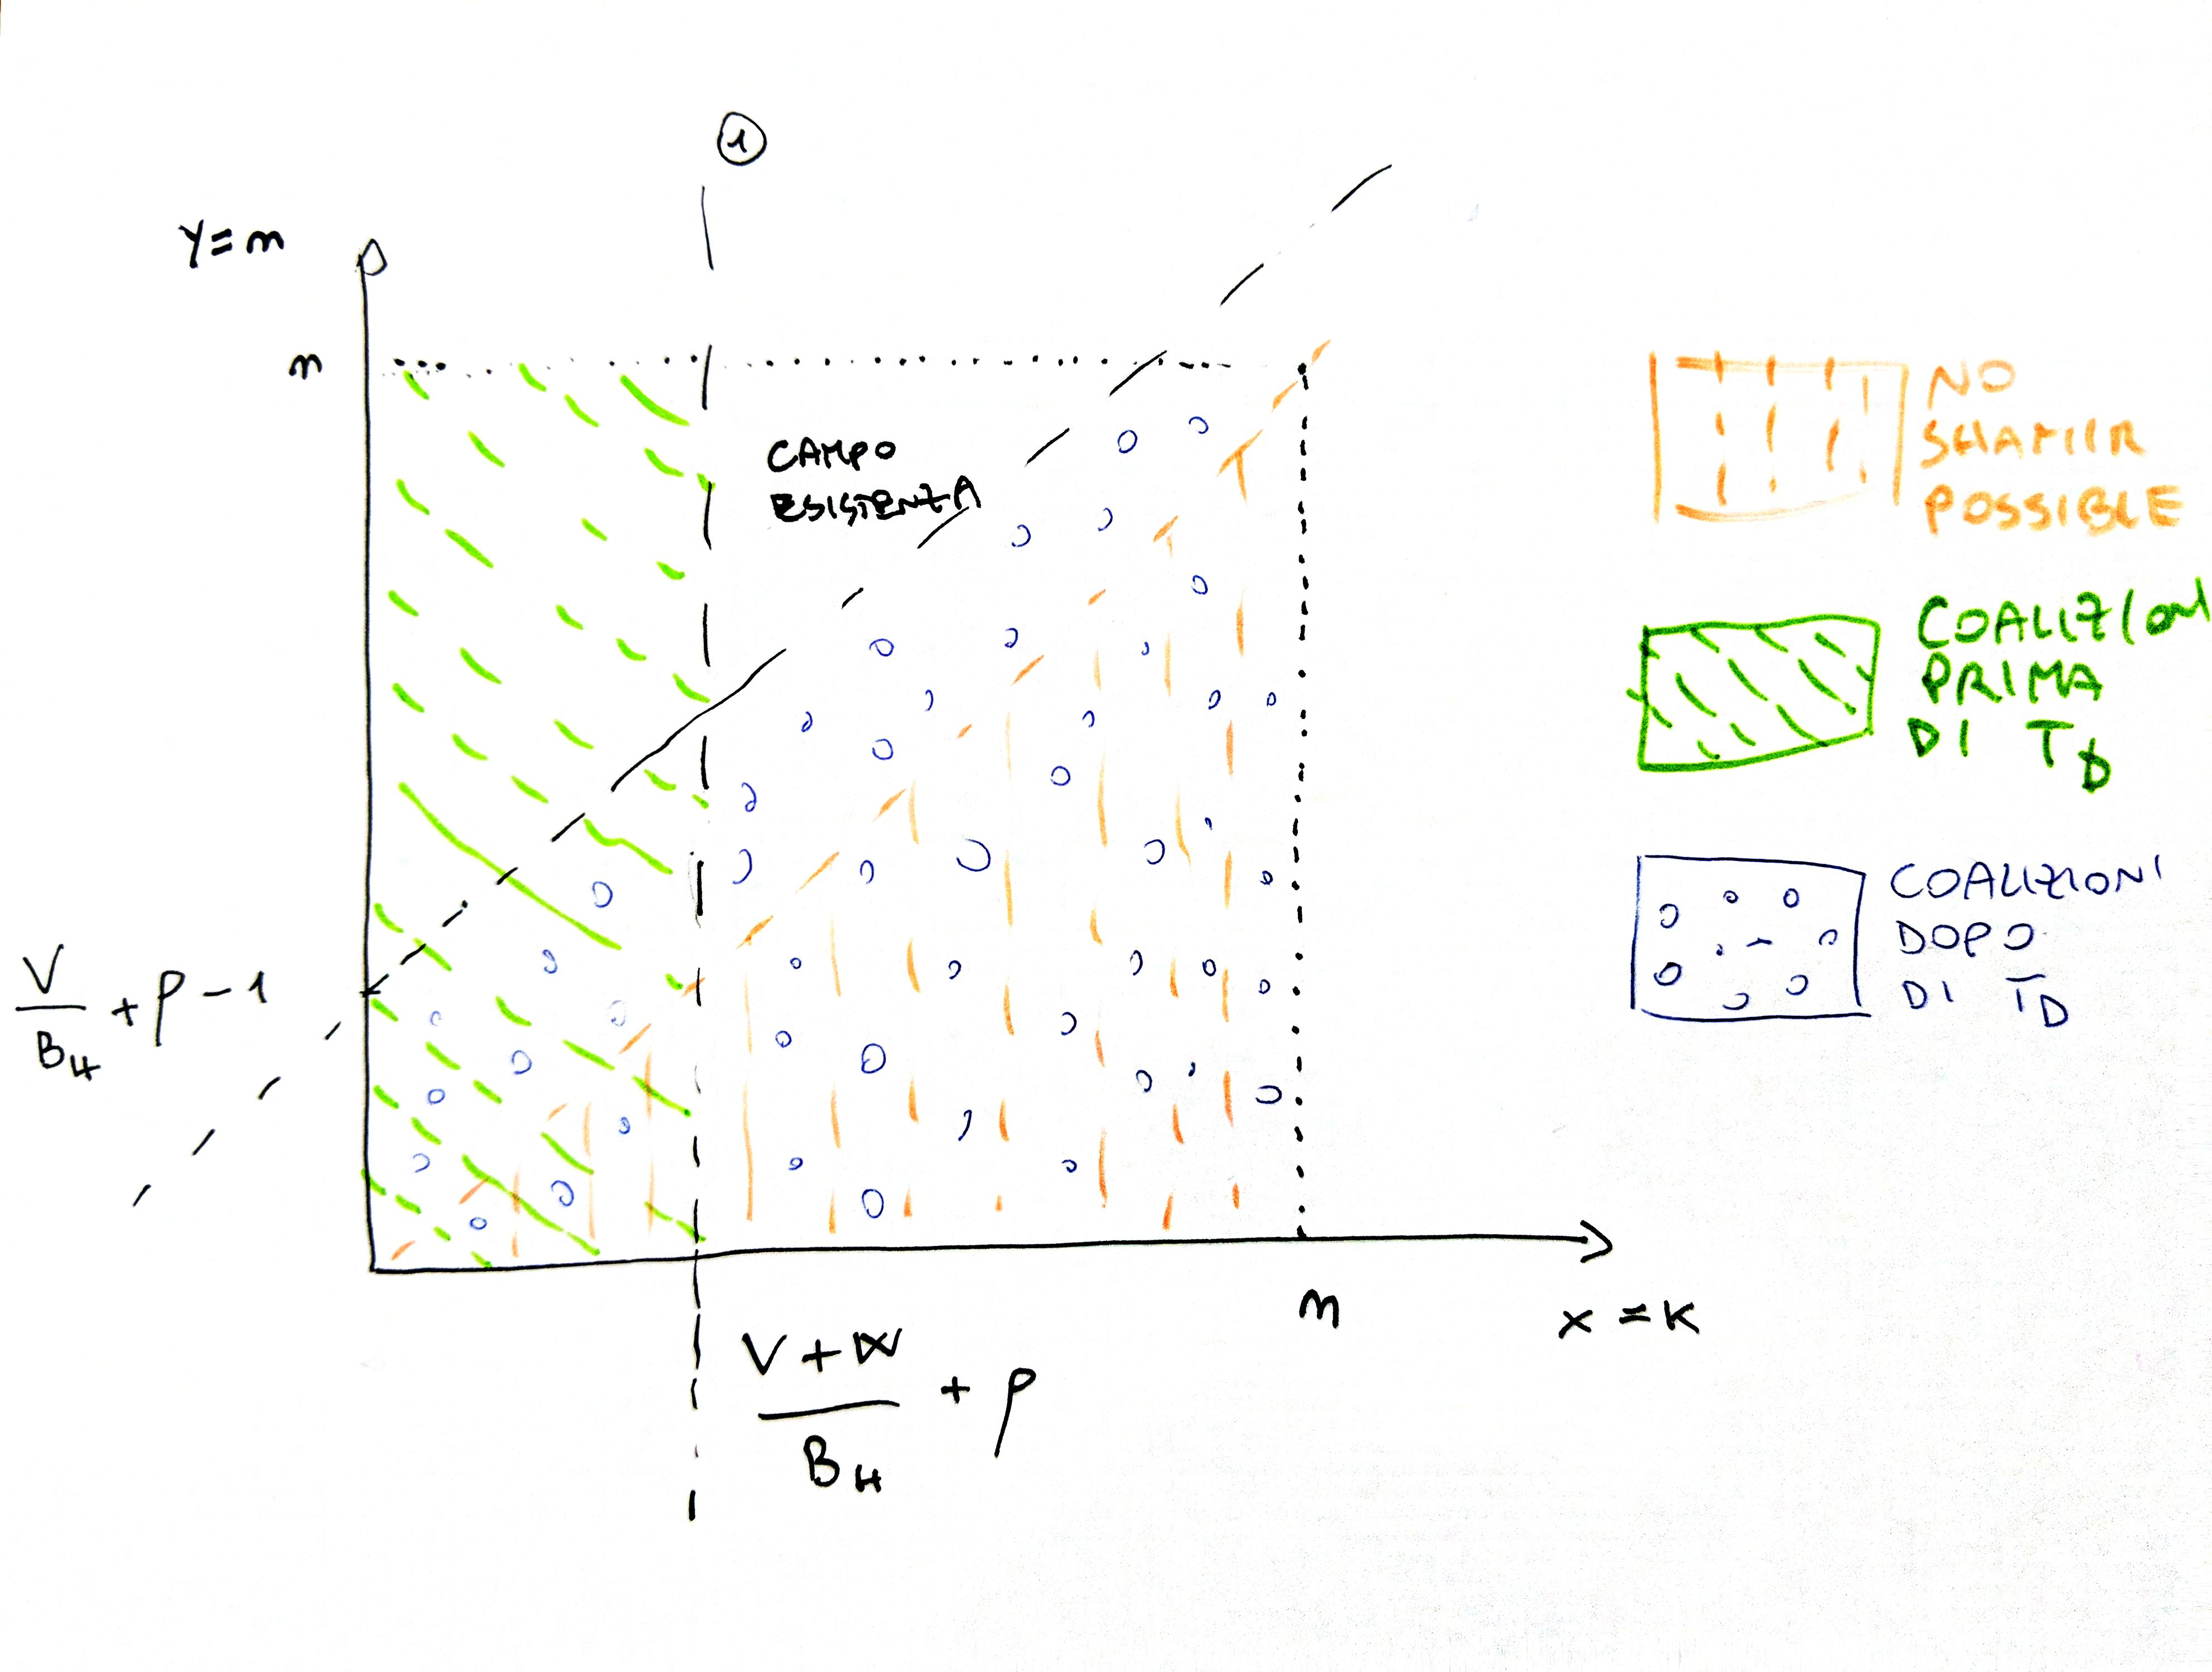
\includegraphics[width=\columnwidth]{fig/constraints}
	\caption{{\em \shortname} constraints}
	\label{fig:constraints}
\end{figure}

due righe per introdurre la rappresentazione grafica dei vincoli e del campo di esistenza del modello, ATTENZIONE TOGLIERE DALLA FIGURA IL CONTRIBUTO DELLE VARIAZIONI
\end{comment}